\section{Abstract}
\small
\textit{Designed to confront the challenges of climate change in the Great Lakes and Oceans, Kamikaze is E-JUST Robotic Club’s entry for the 2025 MATE ROV Competition. Constructed for the purposes of ocean monitoring, marine renewable energy, and ecosystem restoration, it promotes the UN Decade of Ocean Science and propels sustainable developments in underwater exploration. Kamikaze is a product of 47 employees to deliver a robust and mission-ready solution.}

\textit{With only three years of experience, Kamikaze was a large step up from its predecessor Shiro Kaigen, where modularity, sustainability, adaptability and ease of pilot were the main design choices while designing. Kamikaze improves on its predecessor but using a modular aluminum extrusion frame allowing the ease of modification and the specialized tools that can accomplish more specific tasks. Kamikaze also implements a new manipulators design made to grip on a wide range of sizes, a lightweight 3D-printed PETG canister, a seven-thruster propulsion system with six degrees of freedom. In addition to that, Kamikaze also implements new custom-made PCB with STM32 microcontroller, a custom depth sensor, the usage of aluminum wires and built up from ground software with a new custom station to control it.}

\textit{Kamikaze is prepared to perform jobs ranging from documenting Great Lakes shipwrecks to collecting water samples, deploying hydrophones, and maintaining offshore wind farm bases. Accompanied by a custom-built vertical profiling float for autonomous data collecting on ocean health and depth, it becomes a realistic solution for the preservation of great lakes and oceans.}

\normalsize
\begin{figure}[hb!]
    \centering
    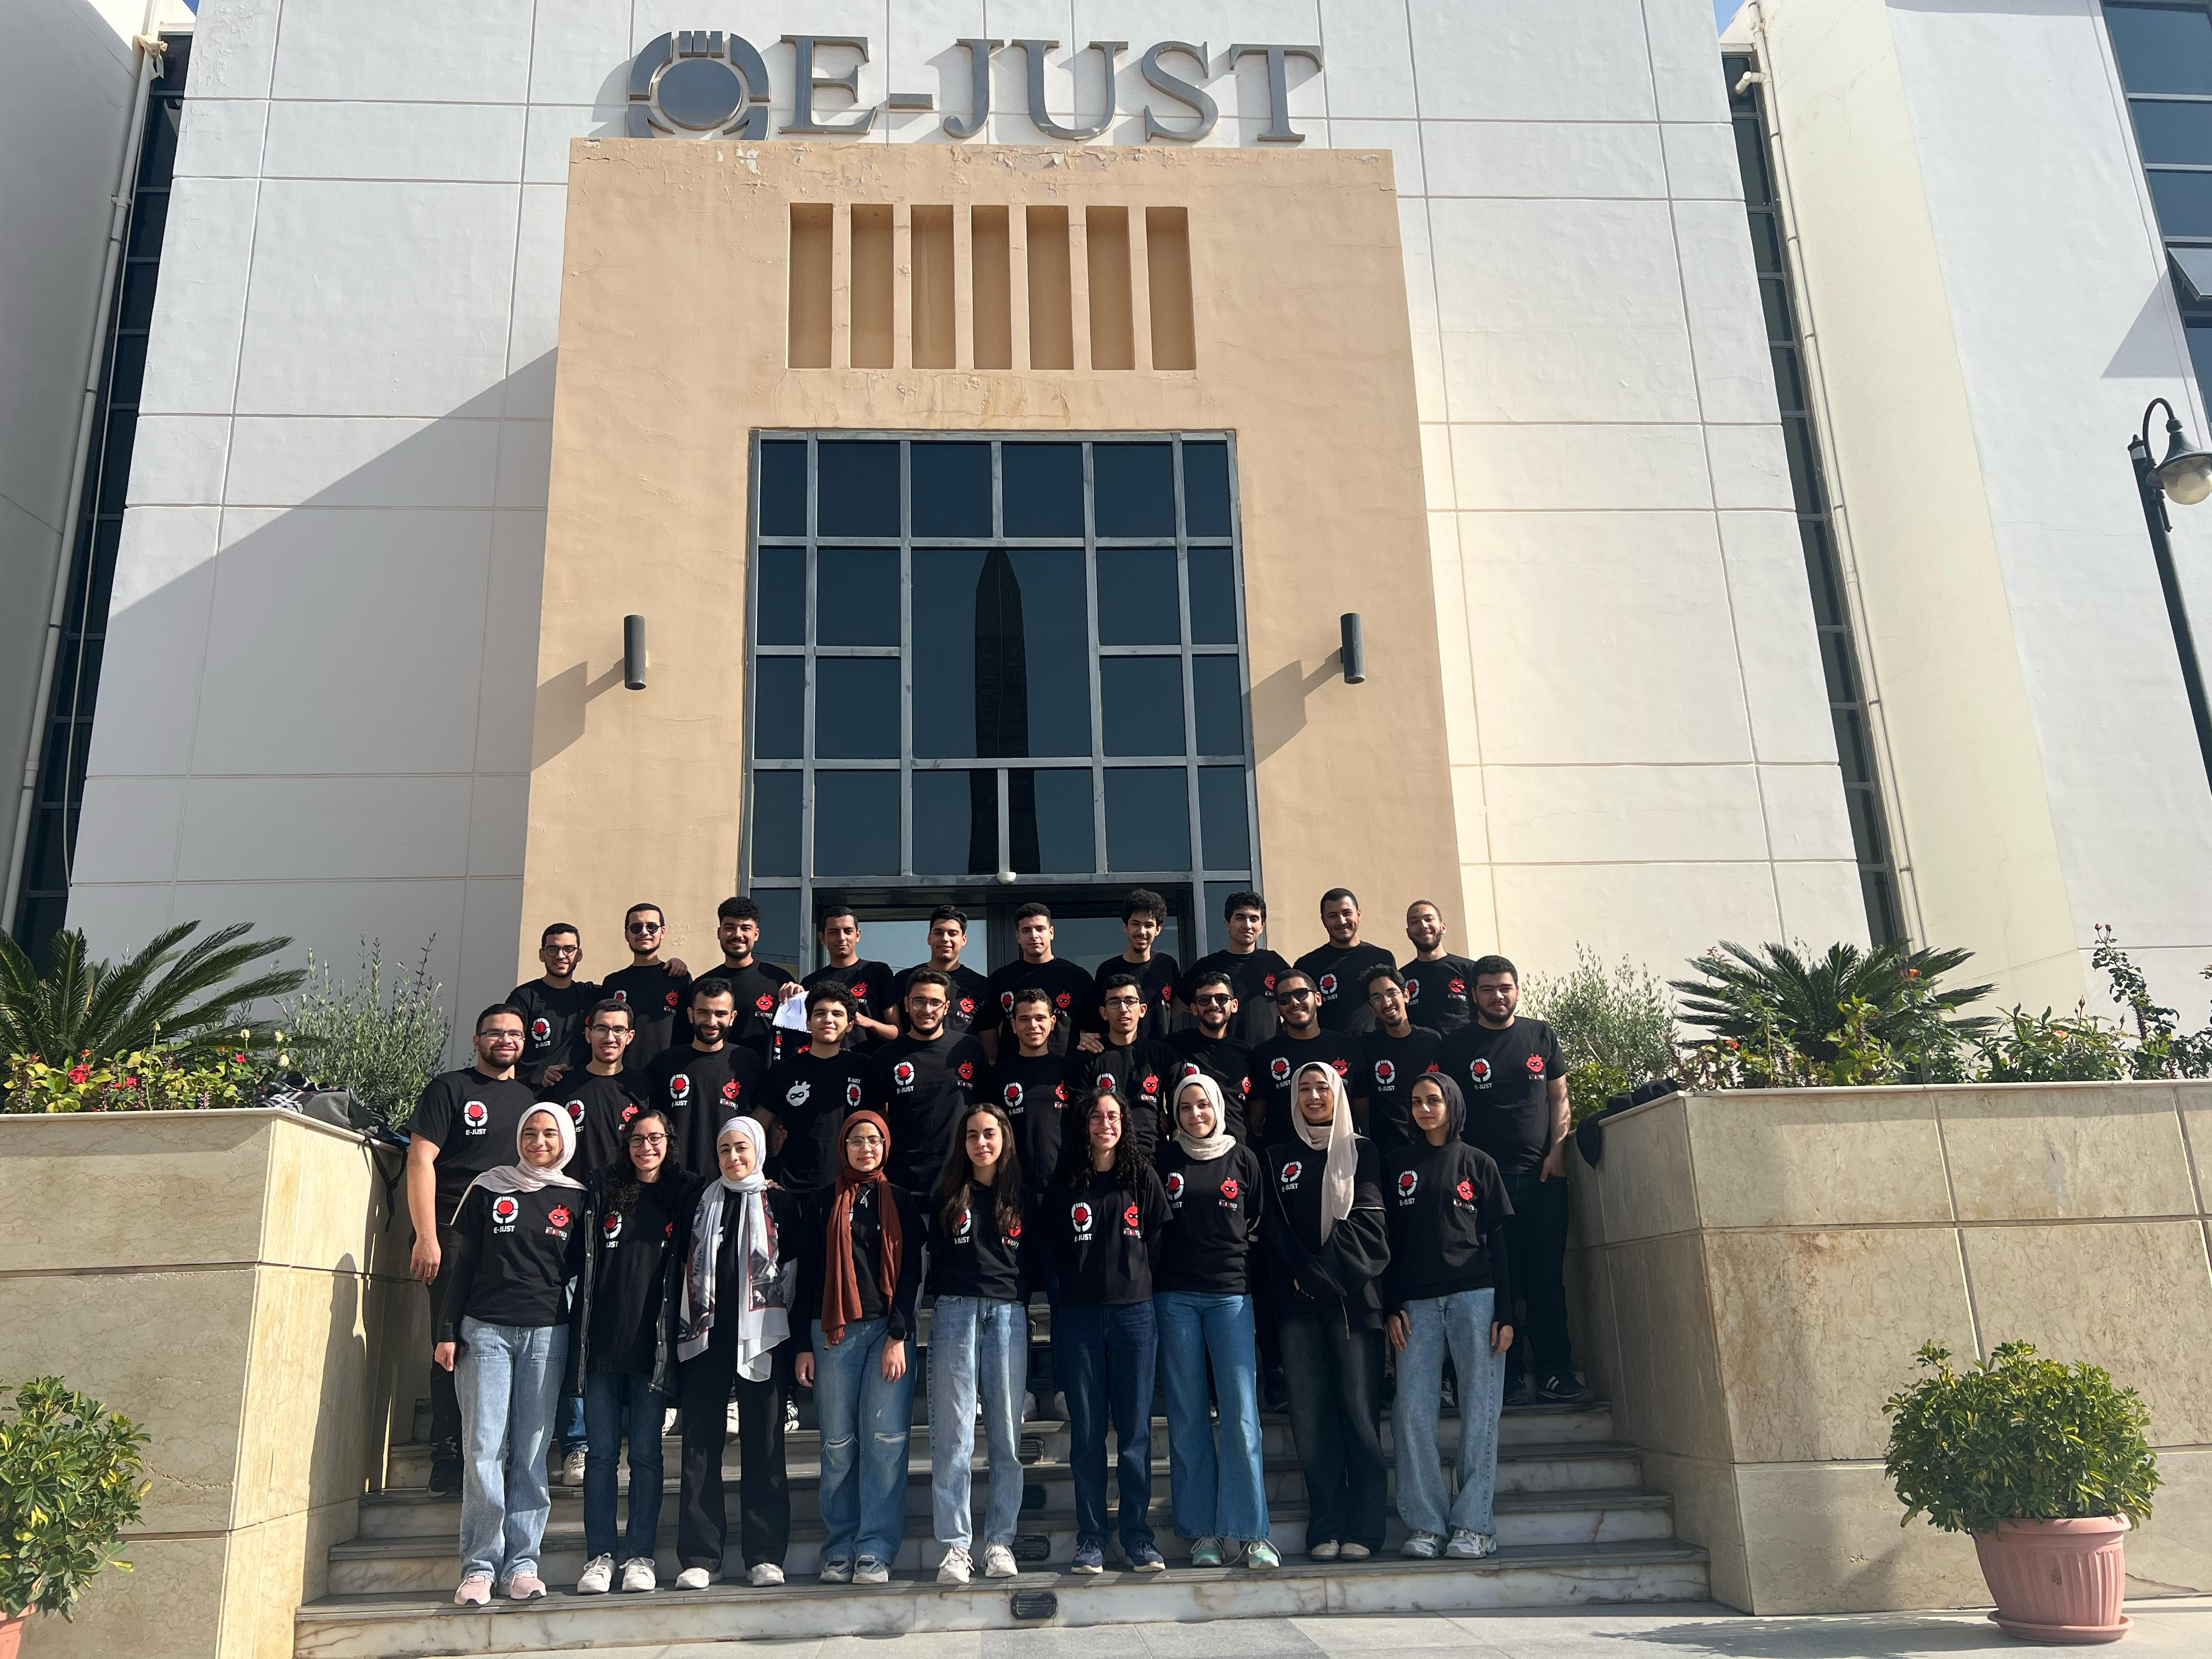
\includegraphics[width=\columnwidth]{Sections/1Abstract/team.jpeg}
    \caption{E-JUST Robotics Club Team.}
    \label{fig:team}
\end{figure}